\section{问题分析}

\subsection{问题一分析}

问题一要求利用无人机FY1投放1枚烟幕干扰弹实现对导弹M1的干扰,核心是在给定投放策略下确定烟幕云团对导弹观测真目标的有效遮蔽时间段,需要建立导弹-云团-目标的几何遮蔽模型,通过分析导弹视线与云团球体的相交关系来判定遮蔽效果,这是一个具有明确物理约束和几何关系的确定性问题。

\subsection{问题二分析}

问题二将真目标从单一圆柱体扩展为圆柱体表面的2000个离散目标点,使问题从确定性计算转变为多目标优化问题,核心挑战是在4维参数空间(飞行方向、速度、投放时间、起爆延迟)内寻找最优解,实现覆盖率最大化和平均遮蔽时间最大化的多目标平衡。

\subsection{问题三分析}

问题三要求利用单架无人机投放3枚烟幕弹实现协同干扰,核心挑战是在6维参数空间(飞行方向、速度、首次投放时间、三个起爆延迟、两个投放间隔)内协调多枚烟幕弹的时空分布,通过逻辑或运算实现协同遮蔽效果,形成连续有效遮蔽并最大化总体干扰时间。

\subsection{问题四分析}

问题四要求设计三架无人机的协同烟幕干扰策略,是一个高维度、强耦合的多无人机协同优化问题,需要在12维参数空间(每架无人机4个决策变量)内寻找最优配置,使三个烟幕云团对2000个目标点实现最大覆盖率和最长平均干扰时间,核心挑战在于处理多云团协同遮蔽效果、时空耦合关系以及严格的约束条件。

\begin{figure}[htbp]
\centering
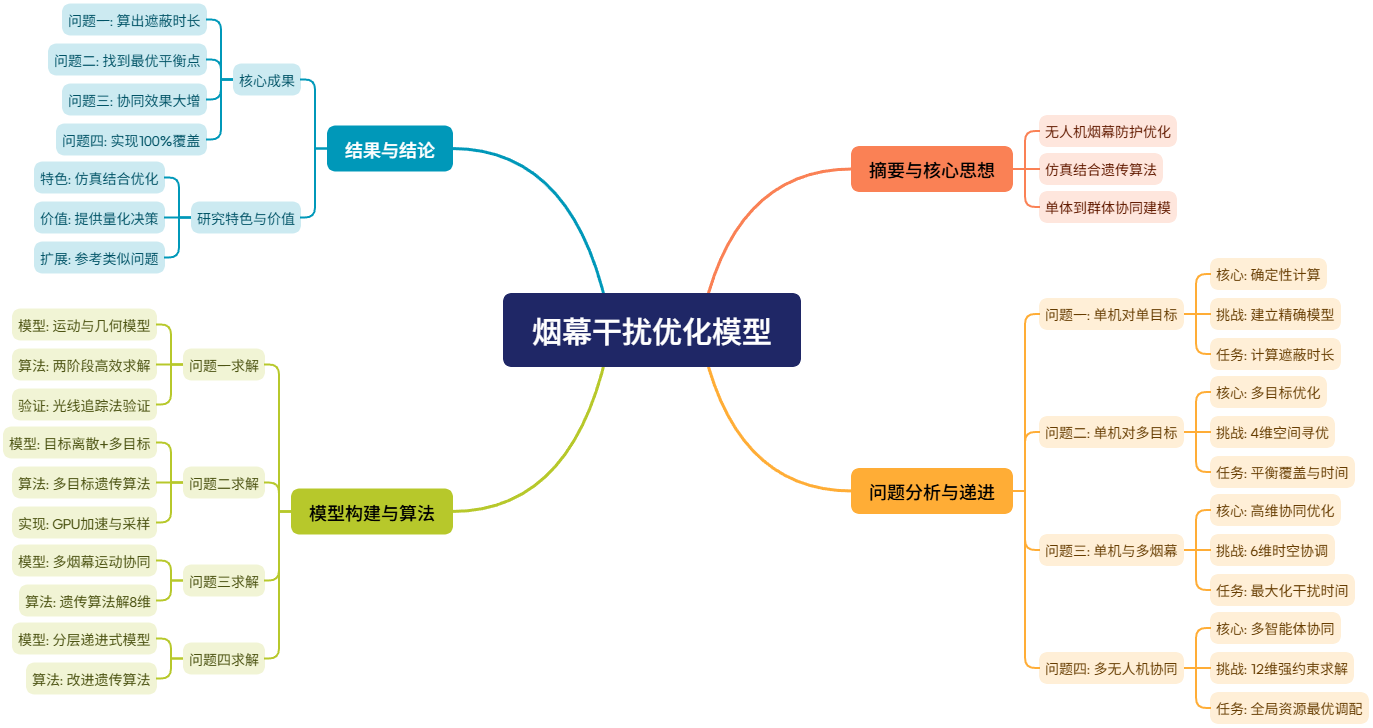
\includegraphics[width=\textwidth]{figures/分析思路.png}
\caption{问题分析思路图}
\label{fig:analysis_approach}
\end{figure}

